\documentclass[a4paper,11pt]{article}
\usepackage[margin=16mm,top=14mm,bottom=15mm]{geometry}
\usepackage[T1]{fontenc}
\usepackage{mathptmx}
\usepackage{microtype,graphicx,amsmath,tikz,caption,titlesec,enumitem}
\usetikzlibrary{arrows.meta}
\usepackage[hidelinks]{hyperref}
\hypersetup{pdftitle={TrajCert: Sharp Risk Identification and Anytime-Valid Certification with Informative Outcome-Resolution Paths},pdfauthor={Salaheddine Naslouby, Mohamed Lachgar, Hamid Hrimech}}
\setlength{\parindent}{0pt}
\setlength{\parskip}{3.5pt}
\linespread{1}
\titleformat{\section}{\large\bfseries}{}{0pt}{}
\titlespacing*{\section}{0pt}{8pt}{4pt}
\captionsetup{hypcap=false,font=small,labelfont=bf,labelsep=period,skip=3pt}
\pagestyle{plain}
\begin{document}\fontsize{10.5}{12.2}\selectfont
\begin{center}
{\fontsize{15}{17}\selectfont\bfseries TrajCert: Sharp Risk Identification and Anytime-Valid\\Certification with Informative Outcome-Resolution Paths\par}
\vspace{5pt}
Salaheddine Naslouby$^{1}$\quad Mohamed Lachgar$^{2}$\quad Hamid Hrimech$^{1}$\par
\vspace{3pt}
{\small $^{1}$Hassan First University, National School of Applied Sciences (ENSA),\\LAMSAD Laboratory, Berrechid, Morocco\par
$^{2}$Cadi Ayyad University, Higher Normal School (ENS),\\L2IS Laboratory, Marrakech, Morocco\par}
\end{center}
\vspace{-4pt}
Risk assessment becomes difficult when harmful outcomes are not always observed. Some events are verified quickly, others only after a delay, and some remain unresolved. When verification depends on the underlying outcome, the observed labels may not represent the full population. Recording only whether verification occurred also discards information carried by its timing.

TrajCert addresses this problem through a risk-identification and certification framework that incorporates the observed outcome-resolution path. A mutual-information sensitivity constraint limits the dependence between harmful outcomes and verification, while the timing information helps determine which risk values remain compatible with the observations. The framework provides sharp population risk bounds and a sequential procedure for certifying risk thresholds under explicit statistical assumptions.

\section{TrajCert Framework and Mathematical Contributions}
\begin{center}
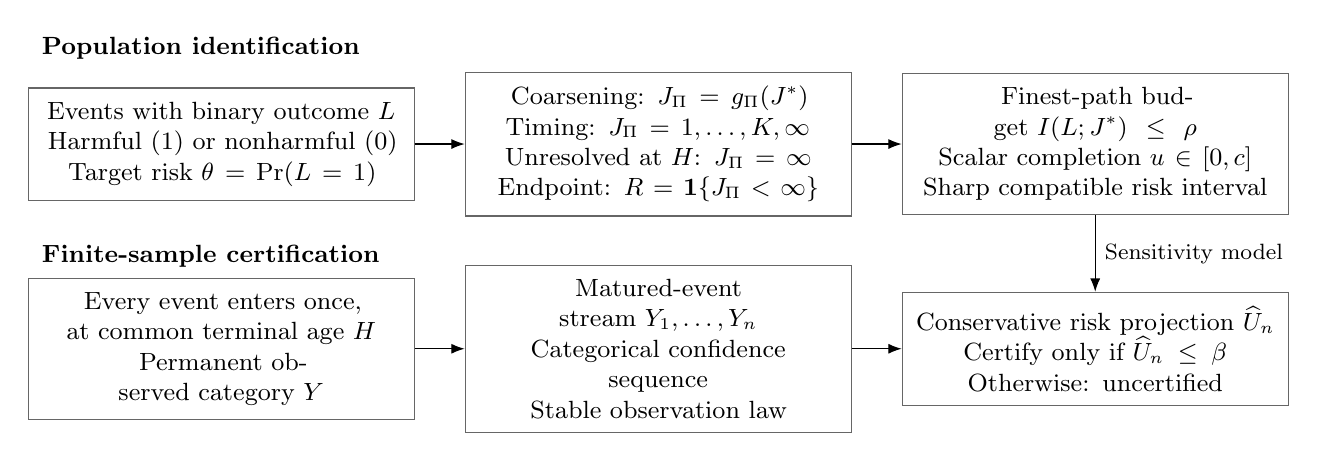
\begin{tikzpicture}[>=Latex,font=\small,every node/.style={align=center},stage/.style={draw=black!60,line width=.4pt,inner sep=5pt,text width=4.55cm,minimum height=1.42cm}]
\node[anchor=west,font=\small\bfseries] at (-2.4,1.22) {Population identification};
\node[stage] (pop) at (0,0) {Events with binary outcome $L$\\Harmful ($1$) or nonharmful ($0$)\\Target risk $\theta=\Pr(L=1)$};
\node[stage] (obs) at (5.55,0) {Coarsening: $J_\Pi=g_\Pi(J^*)$\\Timing: $J_\Pi=1,\ldots,K,\infty$\\Unresolved at $H$: $J_\Pi=\infty$\\Endpoint: $R=\mathbf1\{J_\Pi<\infty\}$};
\node[stage] (id) at (11.1,0) {Finest-path budget $I(L;J^*)\le\rho$\\Scalar completion $u\in[0,c]$\\Sharp compatible risk interval};
\draw[->] (pop)--(obs); \draw[->] (obs)--(id);
\node[anchor=west,font=\small\bfseries] at (-2.4,-1.42) {Finite-sample certification};
\node[stage] (mat) at (0,-2.6) {Every event enters once,\\at common terminal age $H$\\Permanent observed category $Y$};
\node[stage] (cs) at (5.55,-2.6) {Matured-event stream $Y_1,\ldots,Y_n$\\Categorical confidence\\sequence\\Stable observation law};
\node[stage] (cert) at (11.1,-2.6) {Conservative risk projection $\widehat U_n$\\Certify only if $\widehat U_n\le\beta$\\Otherwise: uncertified};
\draw[->] (mat)--(cs); \draw[->] (cs)--(cert); \draw[->] (id.south)--node[right,font=\footnotesize]{Sensitivity model}(cert.north);
\end{tikzpicture}
\captionof{figure}{TrajCert retains outcome-resolution timing and terminal nonresolution when identifying harmful-outcome risk. A confidence sequence and conservative projection extend the population bounds to sequential certification.}
\end{center}
\vspace{-3pt}
\textbf{Sharp risk identification.}
Recent work addresses nonignorable missing outcomes through partial identification and uses callback histories to adjust for nonresponse \cite{dalygrafstein,miao}. TrajCert characterizes harmful-outcome risk through the unknown harmful mass among unresolved events. Under a declared mutual-information constraint, the compatible risk values form a sharp interval determined by a convex one-dimensional information profile. The profile also provides an observable compatibility floor, distinguishing admissible sensitivity assumptions from those contradicted by the observed distribution.

\textbf{The value of resolution timing.}
Resolution timing contributes information that endpoint-only observation discards. TrajCert establishes an exact relationship between timing refinement and the information profile: finer resolution shifts the profile by an observable conditional-information increment. Under a common sensitivity budget, this can tighten the identified risk interval and change whether a risk threshold can be certified.
\[\setlength{\abovedisplayskip}{4pt}\setlength{\belowdisplayskip}{4pt}
 S_f(u)-S_c(u)=I(L;J_f\mid J_c)=\Delta\ge0,\qquad 0\le u\le c.
\]
Here $S_f,S_c$ are fine and coarse information profiles, $J_f,J_c$ their resolution categories at the same horizon ($J_c$ coarsens $J_f$), $c$ the unresolved mass, and $u$ its unknown harmful part. The observable increment $\Delta$ is independent of $u$; risk is $A+u$, with $A$ the resolved harmful mass. The budget $\rho$ is assumed, not learned from unresolved labels.

\textbf{Sequential certification.}
TrajCert extends population identification to sequential monitoring by projecting a categorical confidence sequence onto the compatible risk set. The sequence follows established principles for anytime-valid inference \cite{ramdas}. Conservative upper-risk bounds support certification at successive monitoring checkpoints without relying on a fixed sample size. Time-uniform validity holds under the specified stability, sensitivity, and numerical-enclosure conditions. These require a fixed full law, conditionally stable observed categories, correct resolved labels, and conservative confidence inversion and projection for a prespecified partition.

Observable resolution timing accounts for part of the permitted dependence between outcomes and verification. Under a fixed information budget, this leaves less freedom to assign harmful outcomes to unresolved events, potentially turning an inconclusive risk bound into a certificate.
\newpage
\section{Experimental Validation}
TrajCert was evaluated using synthetic outcome-resolution processes with known harmful-outcome risk. The experiments examine the sharpness of the computed risk bounds, the effect of timing information on certification decisions, and the finite-sample behavior of sequential certification.

\begin{minipage}[t]{.485\linewidth}
\centering
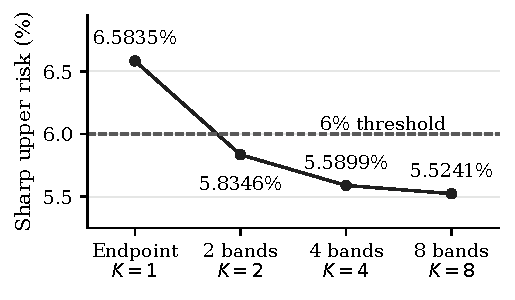
\includegraphics[width=\linewidth]{figures/population.pdf}
\captionof{figure}{Timing changes population certification. Sharp upper risks at $\rho=0.05$ under the timing-and-terminal harmful-late law; the dashed line is $\beta=0.06$. This is a population result.}
\end{minipage}\hfill
\begin{minipage}[t]{.485\linewidth}
\centering
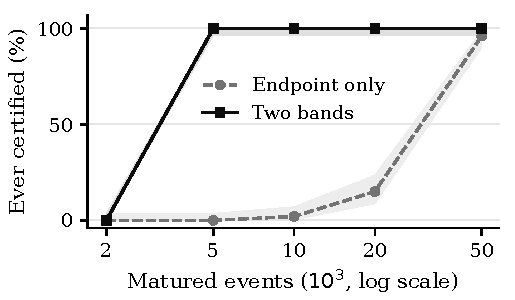
\includegraphics[width=\linewidth]{figures/power.pdf}
\captionof{figure}{Earlier certification under strong timing: $\rho=0.08$, $\beta=0.09$, $\delta=0.05$ per fixed partition. Lines join checkpoint rates; shading gives exact 95\% binomial intervals (100 independent streams per cell).}
\end{minipage}

\textbf{Timing changes the attainable risk decision.}
At the 6\% risk threshold, endpoint-only observation leaves the upper risk above the certification boundary. Retaining two timing bands is sufficient to cross that boundary, with further refinement tightening the population bound to 5.52\%.

\textbf{Earlier certification with informative timing.}
Informative resolution timing also improves finite-sample certification. Under the strong-timing scenario, the two-band procedure certifies all 100 simulated streams by 5,000 matured events, while endpoint-only analysis certifies none at that horizon and reaches 96 of 100 by 50,000 events. The contrast illustrates how timing information can make certification available substantially earlier under favorable conditions. Exact 95\% binomial intervals are $[96.38\%,100\%]$ for 100/100, $[0\%,3.62\%]$ for 0/100, and $[90.07\%,98.90\%]$ for 96/100. These quantify Monte Carlo certification probability; partition comparisons share streams.

At the stricter 7\% risk threshold, endpoint-only analysis records no certifications through 50,000 matured events, whereas the two-band procedure certifies all 100 streams by that horizon. At $\rho=0.08$, the corresponding population upper risks are 7.96\% and 5.91\%: timing changes population certifiability.

\textbf{When timing is useful.}
A matched control retains the strong-timing law's endpoint masses but removes informative resolution timing. The population bounds then coincide. At 50,000 matured events, endpoint-only analysis certifies 94/100 streams and the two-band procedure 28/100. Without informative timing, finer partitions can increase finite-sample uncertainty and computational cost without improving certification. Population-bound refinement therefore does not guarantee higher finite-sample power.

\textbf{Numerical and statistical validation.}
Numerical validation agrees with an independent population-risk oracle across 280 cases, with maximum upper-bound discrepancy below $4.615\times10^{-13}$. Seven additional 500-stream scenarios record one violation in each of two scenarios and zero in the other five, consistent with the statistical construction. These diagnostics do not establish unconditional numerical validity.

\section{Conclusion}
TrajCert establishes how information contained in outcome-resolution timing can improve risk identification and certification under incomplete verification. Its sharp bounds and refinement identity explain when timing changes the admissible risk set, while the sequential procedure enables certification under explicit validity conditions. Synthetic experiments demonstrate both certification decisions unavailable to endpoint-only analysis and substantially earlier certification when timing is informative.

These results depend on the declared sensitivity model and stable observation conditions; implementation-level guarantees require conservative numerical confidence inversion and projection.

\vspace{-3pt}
\renewcommand{\refname}{References}
\begin{thebibliography}{3}
\fontsize{9.5}{10.5}\selectfont\setlength{\itemsep}{1pt}\setlength{\parskip}{0pt}
\bibitem{dalygrafstein} D. Daly-Grafstein and P. Gustafson (2026). Partial identification with categorical data and nonignorable missing outcomes. \emph{Canadian Journal of Statistics} 54(3), e70037.
\bibitem{miao} W. Miao, X. Li, P. Zhang and B. Sun (2025). A stableness of resistance model for nonresponse adjustment with callback data. \emph{JRSS Series B: Statistical Methodology} 87(2), 433--456.
\bibitem{ramdas} A. Ramdas, P. Gr\"unwald, V. Vovk and G. Shafer (2023). Game-theoretic statistics and safe anytime-valid inference. \emph{Statistical Science} 38(4), 576--601.
\end{thebibliography}
\end{document}